\section{Horizontal tracer advection}
\label{sec:advection}

Following \textcite{schaer2002}, a tracer is transported above the orography by solving the advection equation for a prescribed horizontal wind.  This challenges the accuracy of the advection scheme in the presence of grid distortions.
The wind profile, terrain profile and initial tracer field are shown in Figure~\ref{fig:advection:initial}.

\subsection{Specification}
The domain is \SI{300}{\kilo\meter} wide and \SI{25}{\kilo\meter} high.  The terrain is wave-shaped, specified by the surface height $\surface$ such that
\begin{subequations}
\label{eqn:advection:schaerCos}
\begin{align}
	\surface(x) &= \cos^2 \left( \frac{\pi x}{\lambda} \right) \surface^\star
%
	\intertext{where}
%
	\surface^\star(x) &= \left\{ \begin{array}{l l}
		h_0 \cos^2 \left( \frac{\pi x}{2a} \right) & \quad \text{if $| x | < a$} \\
		0 & \quad \text{otherwise}
	\end{array} \right.
\end{align}
\end{subequations}
where $a = \SI{25}{\kilo\meter}$ is the mountain half-width, $h_0 = \SI{3}{\kilo\meter}$ is the maximum mountain height, and $\lambda = \SI{8}{\kilo\meter}$ is the wavelength.  On the SLEVE grid, the large-scale component $\surface_1$, as described in section~\ref{sec:theory:tf}, is given by
\begin{align}
	\surface_1(x) &= \frac{1}{2}\surface^\star(x)
\end{align}
and $s_1 = \SI{15}{\kilo\meter}$ is the large scale height, and $s_2 = \SI{2.5}{\kilo\meter}$ is the small scale height.  The optimisation of SLEVE by \textcite{leuenberger2010} is not used, so the exponent $n = 1$.

For comparison, the same tests were performed with no orography, such that $\surface = \SI{0}{\kilo\meter}$ everywhere.

The wind is entirely horizontal and is prescribed as
\begin{align}
	u(z) = u_0 \left\{ \begin{array}{l l}
		1 & \quad \text{if $z \geq z_2$} \\
		\sin^2 \left( \frac{\pi}{2} \frac{z - z_1}{z_2 - z_1} \right) & \quad \text{if $z_1 < z < z_2$} \\
		0 & \quad \text{otherwise}
	\end{array} \right.	
\end{align}
where $u_0 = \SI{10}{\meter\per\second}$, $z_1 = \SI{4}{\kilo\meter}$ and $z_2 = \SI{5}{\kilo\meter}$.
This results in a constant wind aloft, and zero flow at \SI{4}{\kilo\meter} and below.
A tracer $\varphi$ is positioned upstream above the height of the terrain.  It has the shape
\begin{align}
	\varphi(x, z) &= \varphi_0 \left\{ \begin{array}{l l}
		\cos^2 \left( \frac{\pi r}{2} \right) & \quad \text{if $r \leq 1$} \\
		0 & \quad \text{otherwise}
	\end{array} \right.
%
\intertext{having radius $r$ given by}
%
	r &= \sqrt{
		\left( \frac{x - x_0}{A_x} \right)^2 + 
		\left( \frac{z - z_0}{A_z} \right)^2
	}
\end{align}
where $A_x = \SI{25}{\kilo\meter}$, $A_z = \SI{3}{\kilo\meter}$ are the horizontal and vertical half-widths respectively, and $\varphi_0 = 1$ is the maximum magnitude of the anomaly.  At $t = \SI{0}{\second}$, the anomaly is centred at $(x_0, z_0) = (\SI{-50}{\kilo\meter}, \SI{9}{\kilo\meter})$ so that the anomaly is upwind of the mountain and well above the maximum terrain height of \SI{3}{\kilo\meter}.  Analytic solutions can be found by adjusting the anomaly centre such that $x_0 = ut$.

\begin{figure}
	\centerfloat
	\input{advection-initial-plot}
	\caption{Vertical cross section of the two-dimensional advection test showing the horizontal wind profile, surface terrain profile and tracer field at $t = \SI{0}{\second}$ on a $\SI{300}{\kilo\meter} \times \SI{25}{\kilo\meter}$ domain.  Adapted from \textcite{schaer2002}.}
	\label{fig:advection:initial}
\end{figure}

\subsection{Discretisation}
The OpenFOAM solver \shellcmd{scalarTransportFoam} was used to implicitly solve the advection equation in flux form
\begin{align}
	\frac{\partial \varphi}{\partial t} + \del \cdot \left( \vect{u} \varphi \right) = 0 \label{eq:advection:continuous}
\end{align}

The time derivative ($\partial \varphi / \partial t$) is solved implicitly using a backward-in-time, second order accurate scheme defined as \autocite{openfoam-progguide}
\begin{align}
	\frac{\partial}{\partial t} \int_V \varphi \diff V = \frac{
		3 \left( \varphi V \right)^{(n)} - 
		4 \left( \varphi V \right)^{(n-1)} + 
		\left( \varphi V \right)^{(n-2)}
	}{2 \Delta t}
\end{align}

Spatial discretisation follows the finite volume method described in section~\ref{sec:theory:fv}, using the upwind-biased advection scheme described in section~\ref{sec:method:discretisation}.
The domain is discretised onto a grid having $300 \times 50$ cells such that $\Delta x = \SI{1}{\kilo\meter}$ and $\Delta \trans{z} = \SI{500}{\meter}$.  Unlike \textcite{schaer2002} who use periodic lateral boundaries, we use a fixed value of 0 at the inlet boundary and zero gradient boundaries elsewhere.
Tests are integrated forward in time for \SI{10000}{\second} with a timestep $\Delta t = \SI{25}{\second}$.

\subsection{Results}
\begin{figure}
	\captionsetup[subfigure]{position=b}
	\centering
	\subcaptionbox{BTF \label{fig:advection:cubicUpwind:btf}}[0.49\textwidth]{\input{advection-btf-schaerCos-cubicUpwindCPCFit-contour-plot}}
	\hfill
	\subcaptionbox{BTF from \textcite{schaer2002} \label{fig:advection:schaer:btf}}[0.49\textwidth]{\vspace{0.43in}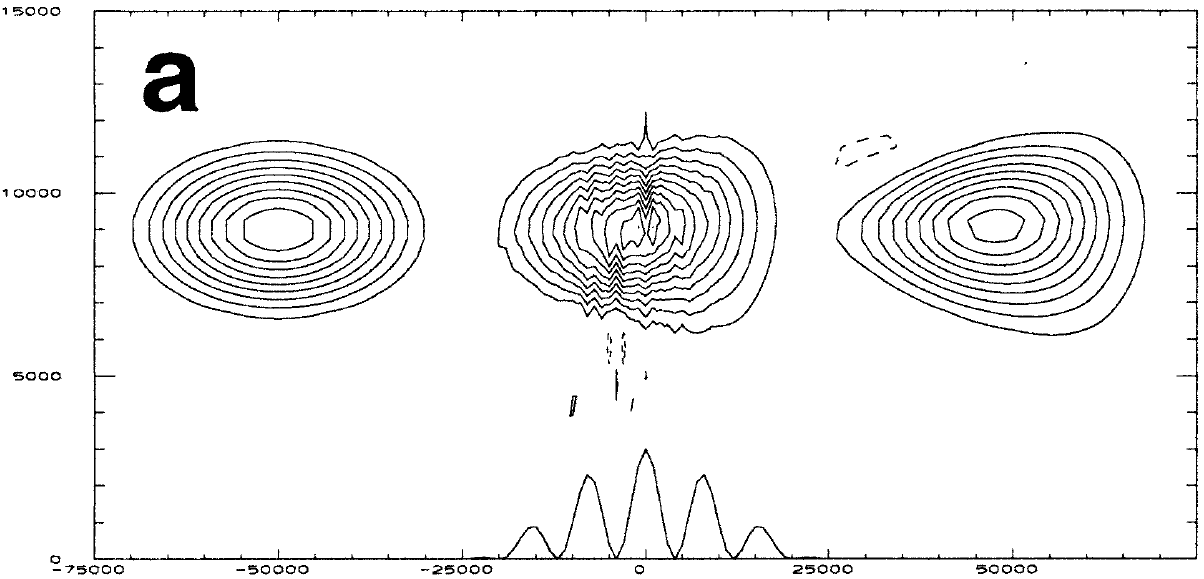
\includegraphics[height=1.2in]{img/schaer-btf-centred.png}}
\\
	\subcaptionbox{SLEVE \label{fig:advection:cubicUpwind:sleve}}[0.49\textwidth]{\input{advection-sleve-schaerCos-cubicUpwindCPCFit-contour-plot}}
	\hfill
	\subcaptionbox{SLEVE from \textcite{schaer2002} \label{fig:advection:schaer:sleve}}[0.49\textwidth]{\vspace{0.43in}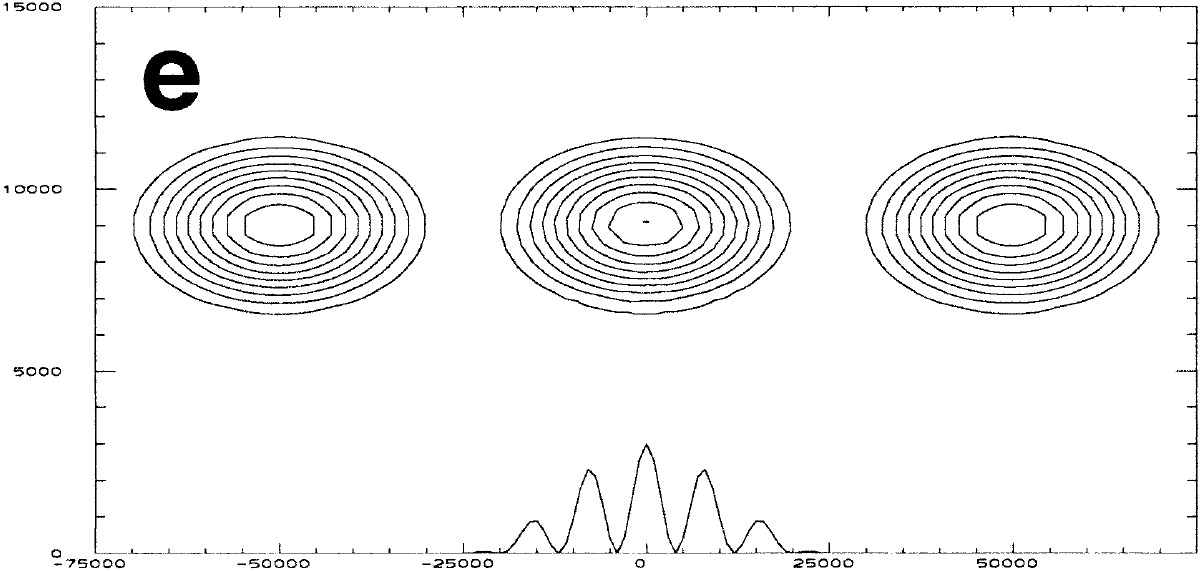
\includegraphics[height=1.2in]{img/schaer-sleve-centred.png}}
\\
	\subcaptionbox{SnapCol grid \label{fig:advection:cubicUpwind:snapCol}}[0.49\textwidth]{\input{advection-snapCol-schaerCos-cubicUpwindCPCFit-contour-plot}}
	\hfill
	\subcaptionbox{Analytic solution on a regular grid \label{fig:advection:analytic}}[0.49\textwidth]{\input{advection-noOrography-analytic-contour-plot}}
%
	\caption{Horizontally advected tracer contours at $t = \SI{0}{\second}$, \SI{5000}{\second} and \SI{10000}{\second}.  Figures (\protect\subref{fig:advection:cubicUpwind:btf}), (\protect\subref{fig:advection:cubicUpwind:sleve}), and (\protect\subref{fig:advection:cubicUpwind:snapCol}) use the upwind-biased scheme described in section~\ref{sec:method:discretisation}.  Figures (\protect\subref{fig:advection:schaer:btf}) and (\protect\subref{fig:advection:schaer:sleve}) show the results of the second-order centred difference scheme from \textcite{schaer2002}.  Contour intervals are every 0.1.}
	\label{fig:advection:cubicUpwind}
\end{figure}

Results of advection are present in figure~\ref{fig:advection:cubicUpwind}.
On the BTF grid, the tracer suffers from distortion over the mountain and some artefacts just above the mountain remain as the tracer moves over it.  Comparing figures~\ref{fig:advection:cubicUpwind:btf} and \ref{fig:advection:schaer:btf}, we see that the tracer retains its shape far better than the result from \textcite{schaer2002} that uses a second-order centred difference scheme.

As seen in figure~\ref{fig:advection:cubicUpwind:sleve}, results on the SLEVE grid are much closer to the analytic solution on a regular grid (figure~\ref{fig:advection:analytic}).  The tracer retains its shape throughout the simulation and does not suffer from any noticeable distortion.  The result agrees with that from \textcite{schaer2002}.

Since the SnapCol grid is entirely regular away from the surface, it is unsurprising that the results (shown in figure~\ref{fig:advection:cubicUpwind:snapCol}) are the same as advection on a regular grid (not shown).  This result agrees with that found by \textcite{good2013}.

\TODO{we could try plotting diffs as done by schaer2002, too.  also, look at min/max values of tracer and discuss lack of monotonicity in advection scheme.}

Error norms were calculated at $t = \SI{10000}{\second}$ by comparing with the analytic solution.  The $\ell^2$ error norm is defined as
\begin{align}
\ell^2 = \sqrt{\frac{\sum \left( \varphi - \varphi_T \right)^2 V}{\sum V}}
\end{align}
where $\varphi$ is the numerical tracer value, $\varphi_T$ is the analytical value and $V$ is the cell volume.  Because the test is two dimensional, the cell volume is equivalent to the cell area.  The resulting errors are summarised in table~\ref{tab:advection:errors}.  Errors on the BTF grid are an order of magnitude greater than the three other grids tested.  The cut cell grid offers only a small error reduction compared to the SLEVE grid.  Even on the BTF grid, the upwind-biased advection scheme is far more tolerant of grid distortions than results of the fourth-order centred scheme from \textcite{schaer2002} (not shown).


